% Helper file that pulls subchapters together.
% Note that \subincludefrom{}{} cannot be nested

% Set initial pages to alpha, so that they do not collide with later Arabic numbering
% in the generated PDF. This won't show in print because page numbers aren't displayed
% until later. But you will be able to print the title page by printing page 'a', which
% would otherwise overlap with page '1', aka the first actual text page.
\pagenumbering{alph}
\maketitle
\subimport{frontmatter/}{colophon}

\frontmatter% In KOMAScript, resets pagenumber, uses Roman numerals etc.
\subimport{frontmatter/}{task}
\subimport{frontmatter/}{authorship_declaration}
\subimport{frontmatter/}{abstract}

%%%%%%%%%%%%%%%%%%%%%%%%%%%%%%%%%%%%%%%%%%%%%%%%%%%%%%%%
% Lists of Content
%%%%%%%%%%%%%%%%%%%%%%%%%%%%%%%%%%%%%%%%%%%%%%%%%%%%%%%%

\tableofcontents

%%%%%%%%%%%%%%%%%%%%%%%%%%%%%%%%%%%%%%%%%%%%%%%%%%%%%%%%
% addchap is KOMA equivalent for \chapter*, but also creates ToC entry, see also
% https://tex.stackexchange.com/a/116085/120853
% Use built-in macro \glossaryname for proper internationalization. With polyglossia, it
% will contain \text<language>{<glossary translation>}, which has been taken care of
% using \pdfstringdefDisableCommands{} in the class file
\addchap{\glossaryname}%

% Print "unsorted" glossaries; these are in fact sorted, but externally using bib2gls.
% These will throw 'Token not allowed in PDF, removing \text<language>' warning.
% Specify title= manually if that gets too annoying.
\printunsrtglossary[
    type=symbols,
    style=symbunitlong,
]
\printunsrtglossary[
    type=numbers,
    style=numberlong,
]
\printunsrtglossary[
    type=subscripts,
    style=mcolalttree,
    nonumberlist,
]
\printunsrtglossary[
    type=abbreviations,
    style=long3colheader,
]

%%%%%%%%%%%%%%%%%%%%%%%%%%%%%%%%%%%%%%%%%%%%%%%%%%%%%%%%
\listoffigures%

\listoftables%

\listofexamples%

\lstlistoflistings%

\chapter{Hello}

\begin{figure}
    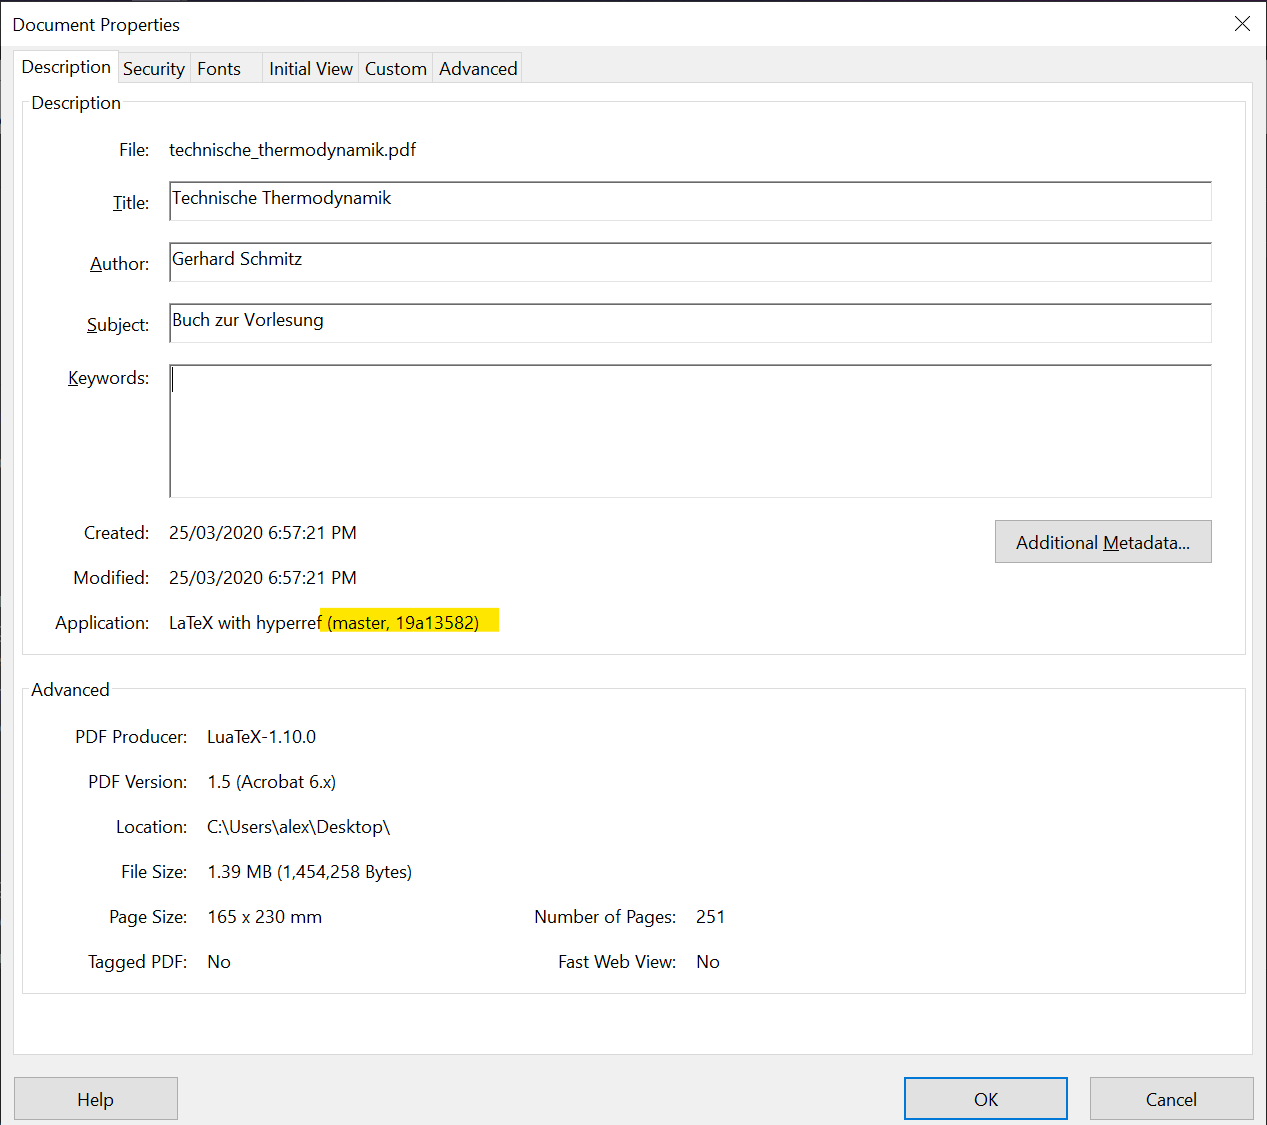
\includegraphics{git_sha_in_pdf_metadata}
    \caption{wow}
\end{figure}

\begin{table}
    \begin{tabular}{ll}
        Hello & World\\
    \end{tabular}
    \caption{rofl}
\end{table}
